% Standard LaTeX template provided by department
\documentclass[11pt]{article}
\usepackage{amsmath,amsbsy,amssymb,verbatim,fullpage,ifthen,graphicx,bm,amsfonts,amsthm,url}
\usepackage{graphicx}
\usepackage{xcolor}
\usepackage{hyperref}
\newcommand{\mfile}[1]  {{\small \verbatiminput{./#1}}} % Jeff Fessler, input matlab file
\newcommand{\tmop}[1]{\ensuremath{\operatorname{#1}}}
%\newcommand*{\qed}{\hfill\ensuremath{\blacksquare}}%
\newcommand{\R}{\mathbb{R}}
\newcommand{\C}{\mathbb{C}}
\newcommand{\Z}{\mathbb{Z}}
\newcommand{\A}{\mathcal{A}}
\newcommand{\minimize}{\operatorname*{minimize\ }}
\newcommand{\maximize}{\operatorname*{maximize}}
\newcommand{\opdet}[1]{\operatorname{\textbf{det}}\left(#1\right)}
\newcommand{\optr}[1]{\operatorname{\textbf{tr}}\left(#1\right)}
\newcommand{\mtx}[1]{\mathbf{#1}}
\newcommand{\vct}[1]{\mathbf{#1}}
\def \lg       {\langle}
\def \rg       {\rangle}
\def \mA {\mtx{A}}
\def \mB {\mtx{B}}
\def \mD {\mtx{D}}
\def \mE {\mtx{E}}
\def \mF {\mtx{F}}
\def \mG {\mtx{G}}
\def \mI {\mtx{I}}
\def \mJ {\mtx{J}}
\def \mL {\mtx{L}}
\def \mU {\mtx{U}}
\def \mS {\mtx{S}}
\def \mV {\mtx{V}}
\def \mW {\mtx{W}}
\def \mLambda {\mtx{\Lambda}}
\def \mSigma {\mtx{\Sigma}}
\def \mX {\mtx{X}}
\def \mY {\mtx{Y}}
\def \mZ {\mtx{Z}}
\def \zero     {\mathbf{0}}
\def \vzero    {\vct{0}}
\def \vone    {\vct{1}}
\def \va {\vct{a}}
\def \vg {\vct{g}}
\def \vm {\vct{m}}
\def \vu {\vct{u}}
\def \vv {\vct{v}}
\def \vw {\vct{w}}
\def \vx {\vct{x}}
\def \vy {\vct{y}}
\def \vz {\vct{z}}
\def \vphi {\vct{\phi}}
\def \vmu {\vct{\mu}}
\def \R {\mathbb{R}}
\def \mC {\mtx{C}}
\def \mB {\mtx{B}}
\def \mA {\mtx{A}}
\def \mX {\mtx{X}}
\def \mY {\mtx{Y}}
\def \mV {\mtx{V}}

%\newcommand{\st}{\operatorname*{\ subject\ to\ }}
\usepackage{algorithm,algpseudocode}
\usepackage{xspace}
\usepackage{hyperref}
% Add a period to the end of an abbreviation unless there's one
% already, then \xspace.
\makeatletter
\DeclareRobustCommand\onedot{\futurelet\@let@token\@onedot}
\def\@onedot{\ifx\@let@token.\else.\null\fi\xspace}

\def\eg{\emph{e.g}\onedot} \def\Eg{\emph{E.g}\onedot}
\def\ie{\emph{i.e}\onedot} \def\Ie{\emph{I.e}\onedot}
\def\cf{\emph{c.f}\onedot} \def\Cf{\emph{C.f}\onedot}
\def\etc{\emph{etc}\onedot} \def\vs{\emph{vs}\onedot}
\def\wrt{w.r.t\onedot} \def\dof{d.o.f\onedot}
\def\etal{\emph{et al}\onedot} \def\st{\emph{s.t}\onedot}
\pagestyle{plain}

\title{{\bf Final Exam, CPSC 8420, Fall 2024}} 
\author{\Large\underline{Collins, Matthew}}% put your name in the LastName, FirstName format
\date{\textbf{\Large\textcolor{red}{Due 12/12/2024, Thursday, 5:59PM EST}}} 
%\date{\today}

\begin{document}
\maketitle

\section*{Problem 1 [15 pts]}
Consider the following problem:
\begin{equation}
\min_{\beta} \frac{1}{2}\|\vy-\mX\beta\|^2_2+\lambda\|\beta\|_1.
\end{equation}
\begin{enumerate}
	\item Prove that if $\lambda\ge\|\mX^T\vy\|_\infty$, then $\beta^*=0$. 
	\item To validate the corretness of the conclusion above, let's find the optimal solution manually via experiment. As $\beta$ is a vector consisting of various elements $\beta[1],\beta[2],\dots,\beta[-1]$, one of the most popular methods to find the optimal solution is so called `coordinate descent' which minimizes a certain coordinate while fixing the rest. For example, we can first fix the rest while optimizing $\beta[1]$, then fix the rest to optimize $\beta[2]$, till $\beta[-1]$. By repeating the process until convergence, the optimal solution will be obtained. Please generate $\lambda\ge\|\mX^T\vy\|_\infty$ and make use of coordinate descent method described above to obtain the optimal $\beta$. It should be a zero vector (or very close to $0$ due to machine precision issue).
\end{enumerate}


\textcolor{red}{P1.1, Answer:}\\

Objective with quadratic loss \(\frac{1}{2}\|\vy - \mX\beta\|_2^2\) and L1-regularization \(\lambda\|\beta\|_1\). At optimal point \(\beta^*\), 
the gradient of quadratic part must balance subdifferential of L1-norm. 

Gradient of quadratic is:

\[
\nabla_\beta \left(\frac{1}{2}\|\vy - \mX\beta\|_2^2 \right) = -\mX^T (\vy - \mX\beta).
\]

For the L1-norm, the subdifferential \(\partial \|\beta\|_1\) at any point \(\beta\) is given by:
\[
[\partial \|\beta\|_1]_j = \begin{cases}
\text{sgn}(\beta_j) & \text{if } \beta_j \neq 0 \\
[-1,1] & \text{if } \beta_j = 0
\end{cases}
\]

At the optimal point \(\beta^*\), the following optimality condition must hold:

\[
\mX^T (\vy - \mX\beta^*) \in \lambda \cdot \partial \|\beta^*\|_1.
\]

Check \(\beta^* = 0\). Then \(\mX\beta^* = 0\), so residual is \(\vy - \mX\beta^* = \vy\). putting in gradient:

\[
\mX^T (\vy - \mX\beta^*) = \mX^T \vy.
\]

for \(\beta^* = 0\) to be optimal:

\[
\mX^T \vy \in \lambda \cdot \partial \|\beta^*\|_1.
\]

since \(\beta^* = 0\), subdifferential is \([-1, 1]^p\). this means:

\[
\|\mX^T \vy\|_\infty \leq \lambda.
\]

Therefore when \(\lambda \geq \|\mX^T \vy\|_\infty\), \(\beta^* = 0\) is optimal solution.\\


\textcolor{red}{P1.2, Answer:}\\

To validate my theoretical result from P1.1, I implemented coordinate descent to find the optimal solution experimentally. 
First, I computed $\|\mX^T\vy\|_\infty \approx 180.30$ and set $\lambda \approx 198.30$ to ensure $\lambda \geq \|\mX^T\vy\|_\infty$. 
Figure~\ref{fig:p1_2_descent} shows the convergence of my coordinate descent algorithm, where the objective value decreases monotonically 
and stabilizes after 3 iterations. My algorithm converged to an optimal solution $\beta^*$ where all components are zero as shown in Figure~\ref{fig:p1_2_output}. 
These experimental results confirm my theoretical conclusion that when $\lambda \geq \|\mX^T\vy\|_\infty$, the optimal solution is indeed the zero vector.\\

\begin{figure}[h]
\centering
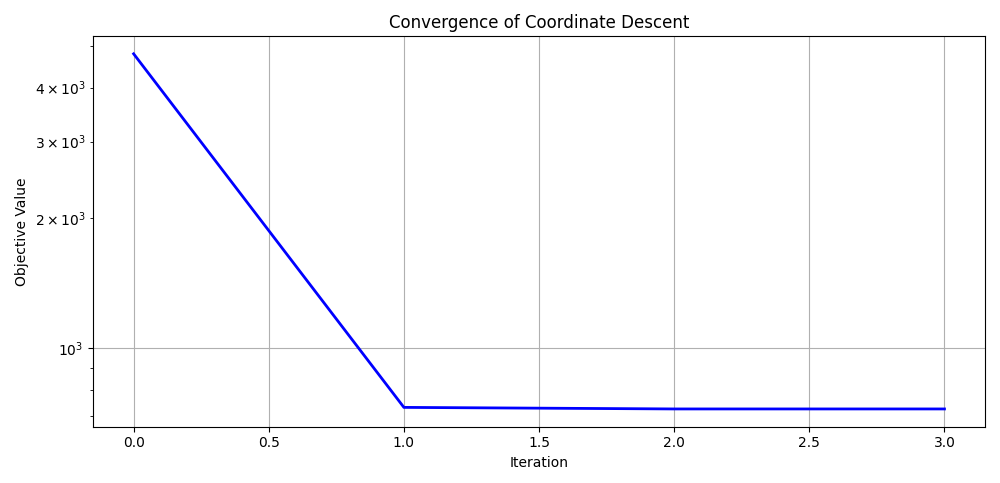
\includegraphics[width=0.8\textwidth]{p1_2_descent.png}
\caption{Convergence of coordinate descent showing objective value vs. iteration.}
\label{fig:p1_2_descent}
\end{figure}

\begin{figure}[h]
\centering
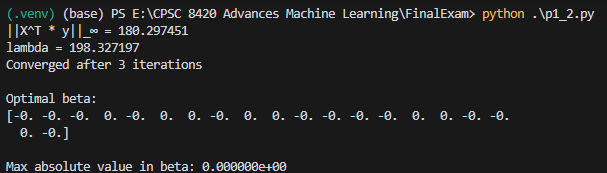
\includegraphics[width=0.8\textwidth]{p1_2_output.png}
\caption{Terminal output showing convergence to zero solution.}
\label{fig:p1_2_output}
\end{figure}



\newpage
\section*{Problem 2 [10 pts]}
\begin{itemize}
	\item For any matrix with SVD decomposition $X=U\Sigma V^T$, define $\|X\|_2=\Sigma(1,1), \|X\|_F=\sqrt{\sum_i\sum_j |x_{ij}|^2}$. Prove that $\|X\|_F\ge \|X\|_2$ and indicate when the equality holds.
	\item Use the fact that $vec(\mA\mX\mB)=(\mB^T\otimes\mA)vec(\mX)$ to find the best solution to $\min\limits_{\mX} \|\mA\mX\mB-\mY\|_F^2$, where $\mA\in\R^{m\times p}, \mX\in\R^{p\times q}, \mB\in\R^{q\times n}, \mY\in\R^{m\times n}$.
\end{itemize}


\textcolor{red}{P2.1, Answer:}\\

For matrix $X$ with SVD $X=U\Sigma V^T$, the singular values $\sigma_i$ are ordered such that 

$\sigma_1 \geq \sigma_2 \geq ... \geq \sigma_r \geq 0$ where $r$ is the rank of $X$. 

By definition, $\|X\|_2 = \sigma_1$ and $\|X\|_F = \sqrt{\sum_{i=1}^r \sigma_i^2}$. 

Then:

\[
\|X\|_F^2 = \sum_{i=1}^r \sigma_i^2 = \sigma_1^2 + \sum_{i=2}^r \sigma_i^2 \geq \sigma_1^2 = \|X\|_2^2
\]

Taking square root of both sides gives $\|X\|_F \geq \|X\|_2$. Equality holds if and only if $\sigma_i = 0$ 

for all $i \geq 2$. $X$ is a rank-1 matrix.\\

\textcolor{red}{P2.2, Answer:}\\

Using the property $\|M\|_F^2 = vec(M)^Tvec(M)$ and the given fact $vec(\mA\mX\mB)=(\mB^T\otimes\mA)vec(\mX)$,

rewrite the objective:

\[
\|\mA\mX\mB-\mY\|_F^2 = \|vec(\mA\mX\mB)-vec(\mY)\|_2^2 = \|(\mB^T\otimes\mA)vec(\mX)-vec(\mY)\|_2^2
\]

This is now a standard least squares problem in vector form. 

Let $\mC = \mB^T\otimes\mA$ and $\vy = vec(\mY)$. 

The optimal solution is:

\[
vec(\mX^*) = (\mC^T\mC)^{-1}\mC^T\vy = ((\mB^T\otimes\mA)^T(\mB^T\otimes\mA))^{-1}(\mB^T\otimes\mA)^Tvec(\mY)
\]

Using the properties of Kronecker product: 

$(\mB^T\otimes\mA)^T = \mB\otimes\mA^T$ and $(\mB^T\otimes\mA)(\mB\otimes\mA^T) = (\mB^T\mB)\otimes(\mA\mA^T)$

the solution becomes:

\[
vec(\mX^*) = ((\mB\mB^T)\otimes(\mA^T\mA))^{-1}(\mB\otimes\mA^T)vec(\mY)
\]


\newpage

\section*{Problem 3 [25 pts]}
Please find \textit{USArrests} dataset online and 
\begin{itemize}
	\item Implement your own program to reproduce the image on page 16/26 of `PCA' slides on Canvas (if yours is flipped up and down, (or) left and right from the slide, it is totally Okay).
	\item For each state, out of 4 features, randomly mask one and assume it is missing (therefore you have your own $\Omega$ and $X$). Please write a program following what we discussed in class (you may refer to ProximalGradientDescent.pdf on Canvas) to optimize  
		\begin{equation}
		\min_{Z} \frac{1}{2}\|P_\Omega(X-Z)\|_F^2+\|Z\|_*,
	\end{equation}
	and plot the objective vs. iteration to demonstrate the algorithm will decrease the function.
\end{itemize}

\textcolor{red}{P3.1, Answer:}\\

See Figure~\ref{fig:p3_1} for the PCA plot of US Arrests Data.

\begin{figure}[h]
	\centering
	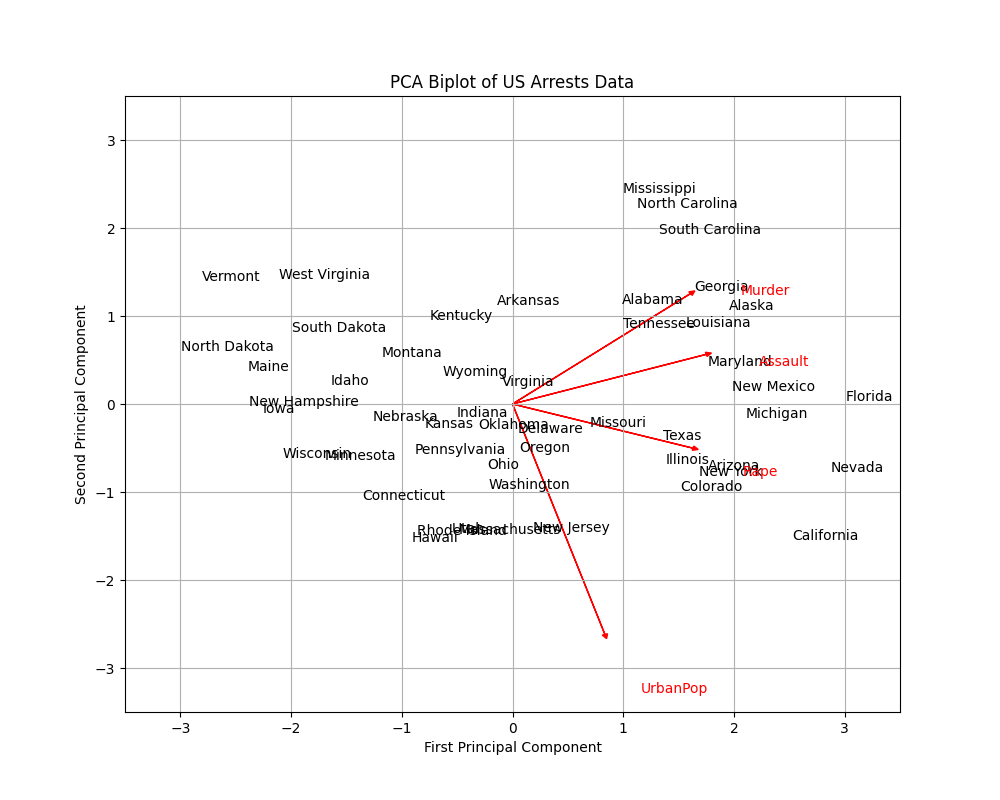
\includegraphics[width=0.8\textwidth]{p3_1.png}
	\caption{PCA Biplot of US Arrests Data}
	\label{fig:p3_1}
	\end{figure}

\textcolor{red}{P3.2, Answer:}\\

See Figure~\ref{fig:p3_2} for the objective vs. iteration plot.

\begin{figure}[h]
	\centering
	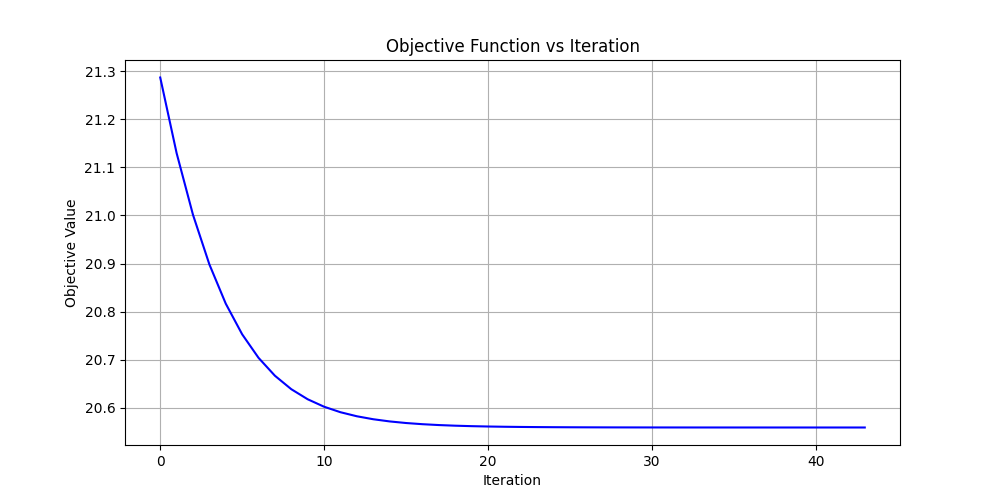
\includegraphics[width=0.8\textwidth]{p3_2.png}
	\caption{Objective vs. Iteration}
	\label{fig:p3_2}
	\end{figure}

\clearpage	
\newpage

\section*{Problem 4 [15 pts]}
Please reproduce Figure (14.29) in \href{https://hastie.su.domains/ElemStatLearn/}{The Elements of
	Statistical Learning} with your own codes. You are NOT allowed to call `spectral clustering' function built-in python or matlab.
	
See Figure~\ref{fig:p4} for the spectral clustering result.
	
\begin{figure}[h]
	\centering
	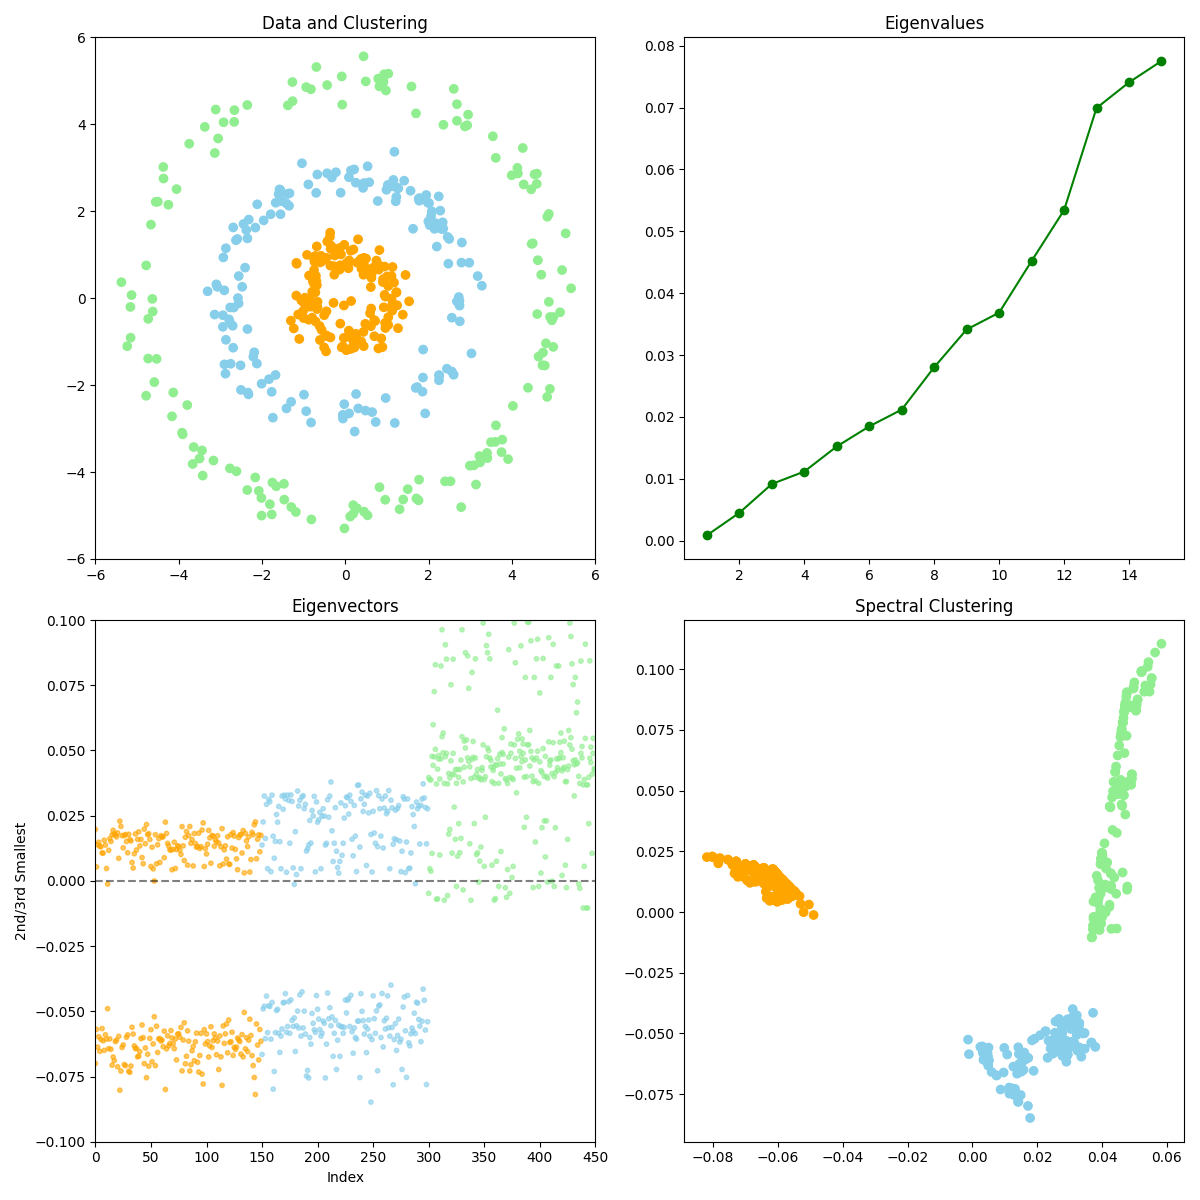
\includegraphics[width=0.8\textwidth]{p4.png}
	\caption{Spectral Clustering}
	\label{fig:p4}
	\end{figure}

\newpage
\section*{Problem 5 [20 pts]}
For Logistic Regression, assume each data $\vx_i\in\R^{100}$. If the label is $\pm1$,  the objective is:
\begin{equation}
\min_\vw	\sum_{i=1}^{m}\log(1+\exp(-y_i\vw^T\vx_i))
\end{equation}
while if the label is $\{1,0\}$ the objective is:
\begin{equation}
	\min_\vw	\sum_{i=1}^{m}\log(1+\exp(\vw^T\vx_i))-y_i\vw^T\vx_i
\end{equation}
\begin{itemize}
	\item Write a program to show that the optimal solutions to the two cases  are the same by making use of gradient descent method where $m=100$ (please carefully choose the stepsize as we discussed in class). You can generate two class samples, one class's label is 1 and the other is -1 or 0 corresponding to the two formulations respectively. You can initialize $\vw$ as $\vzero$.
	\item Consider the case where class label is $\{1,0\}$ and $P(y=1|\vx,\vw)=\frac{1}{1+\exp(-\vw^T\vx)}$, the maximum likelihood function is $p^y(1-p)^{1-y}$. Please prove optimal $p^*=y$. If we use Mean Square Error instead of cross entropy: $\min\limits_p \frac{1}{2}(y-p)^2$, and assume groundtruth $y=1$ and our initial guess weight $\vw$ result in $p$ very close to 0, if we optimize this objective by making use of gradient descent method, what will happen? Please explain why.
	\item For the second objective where the label is $\{1,0\}$, implement Newton method (with unit stepsize) where $m=100$.  Compare with gradient descent method (constant stepsize) and plot objective versus \textbf{iteration} in one figure.
	\item Still consider the second formulation. Please write a stochastic gradient descent version (you may set the stepsize as $1/(t+1)$ where $t=0,1,2,\dots$) and compare those two methods (gradient descent vs. stochastic gradient descent) for $m=[100000,10000,1000,100]$ by plotting objective changes versus \textbf{time consumption} respectively.
\end{itemize}

\textcolor{red}{P5.1, Answer:}\\

See Figure~\ref{fig:p5_1} for the gradient descent for logistic regression.\\


\begin{figure}[h]
	\centering
	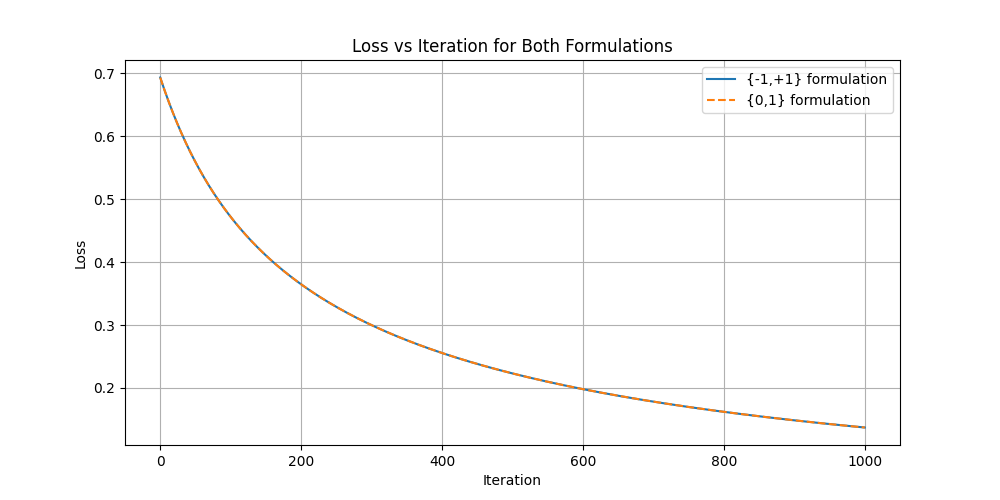
\includegraphics[width=0.8\textwidth]{p5_1.png}
	\caption{Gradient Descent for Logistic Regression}
	\label{fig:p5_1}
	\end{figure}

\begin{figure}[h]
	\centering
	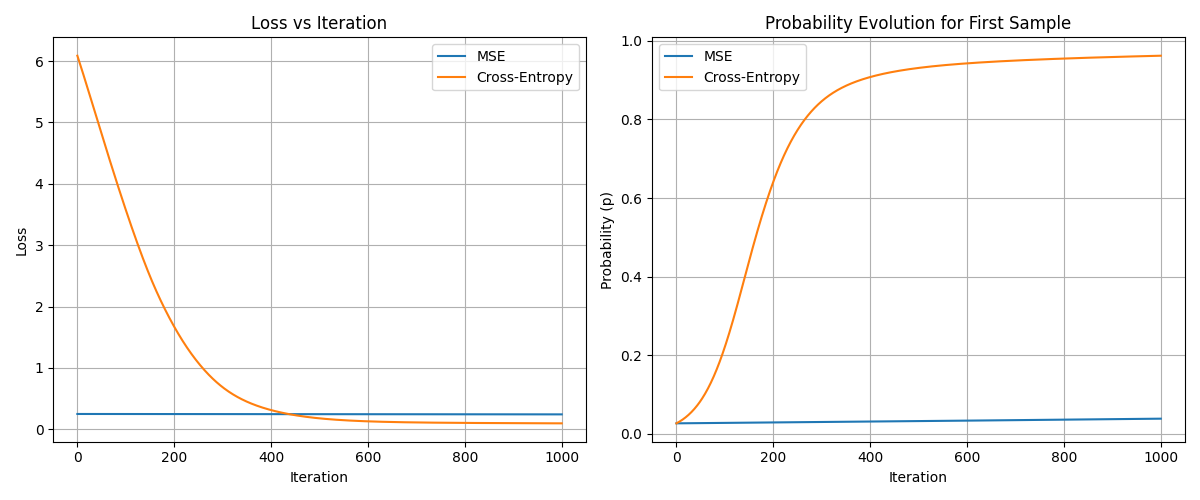
\includegraphics[width=0.8\textwidth]{p5_2.png}
	\caption{MSE vs Cross-Entropy for Logistic Regression}
	\label{fig:p5_2}
	\end{figure}

\textcolor{red}{P5.2, Answer:}\\

When using Mean Square Error (MSE) instead of cross-entropy for logistic regression with ground truth $y=1$ and initial weights giving $p\approx0$, the optimization 
will get stuck and fail to converge to the correct probability. As shown in Figure~\ref{fig:p5_2}, the MSE optimization remains trapped near $p \approx 0$ throughout 
all iterations, while cross-entropy successfully converges to $p \approx 1$. This occurs because the gradient of MSE contains a term $p(1-p)$ multiplied by $(y-p)$. 
When $p$ is very close to 0 and $y=1$, this gradient becomes approximately $0 \cdot 1 \cdot 1 = 0$, resulting in vanishingly small updates to the weights.

\newpage
\textcolor{red}{P5.3, Answer:}\\

As shown in Figure~\ref{fig:p5_3}, Newton's method demonstrates significantly faster convergence compared to gradient descent for logistic regression with {0,1} labels. 
The Newton method achieves optimal loss within just a few iterations due to its quadratic convergence rate, leveraging both gradient and Hessian 
information to make more informed optimization steps. In contrast, gradient descent exhibits a much slower, linear convergence rate, requiring 
hundreds of iterations to approach the same minimum value. This difference in convergence speed is expected theoretically, as Newton's method approximates 
the objective function locally with a quadratic model at each iteration, allowing it to adapt its step size and direction optimally.

\textcolor{red}{P5.4, Answer:}\\

Figure~\ref{fig:p5_4} compares the convergence behavior of gradient descent (GD) and stochastic gradient descent (SGD) for logistic regression with varying sample sizes m. 
For small datasets (m=100, 1000), both methods perform similarly in terms of time efficiency. However, as the sample size increases to m=10000 and m=100000, 
SGD demonstrates significantly faster convergence than GD, reaching lower loss values in less time. This illustrates SGD's computational advantage over GD for 
large-scale problems, as each SGD iteration processes only a small batch of samples rather than the entire dataset.


\begin{figure}[h]
	\centering
	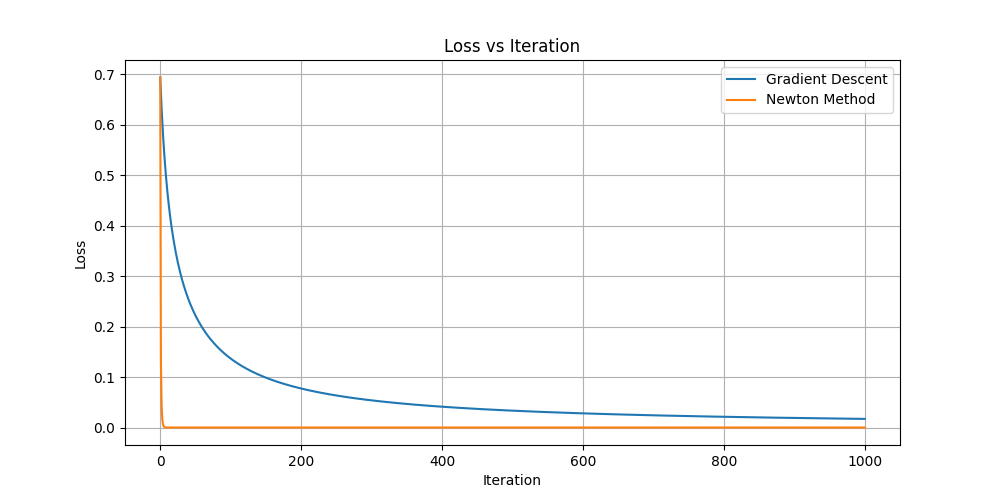
\includegraphics[width=0.8\textwidth]{p5_3.png}
	\caption{Newton vs. Gradient Descent}
	\label{fig:p5_3}
	\end{figure}

\begin{figure}[h]
	\centering
	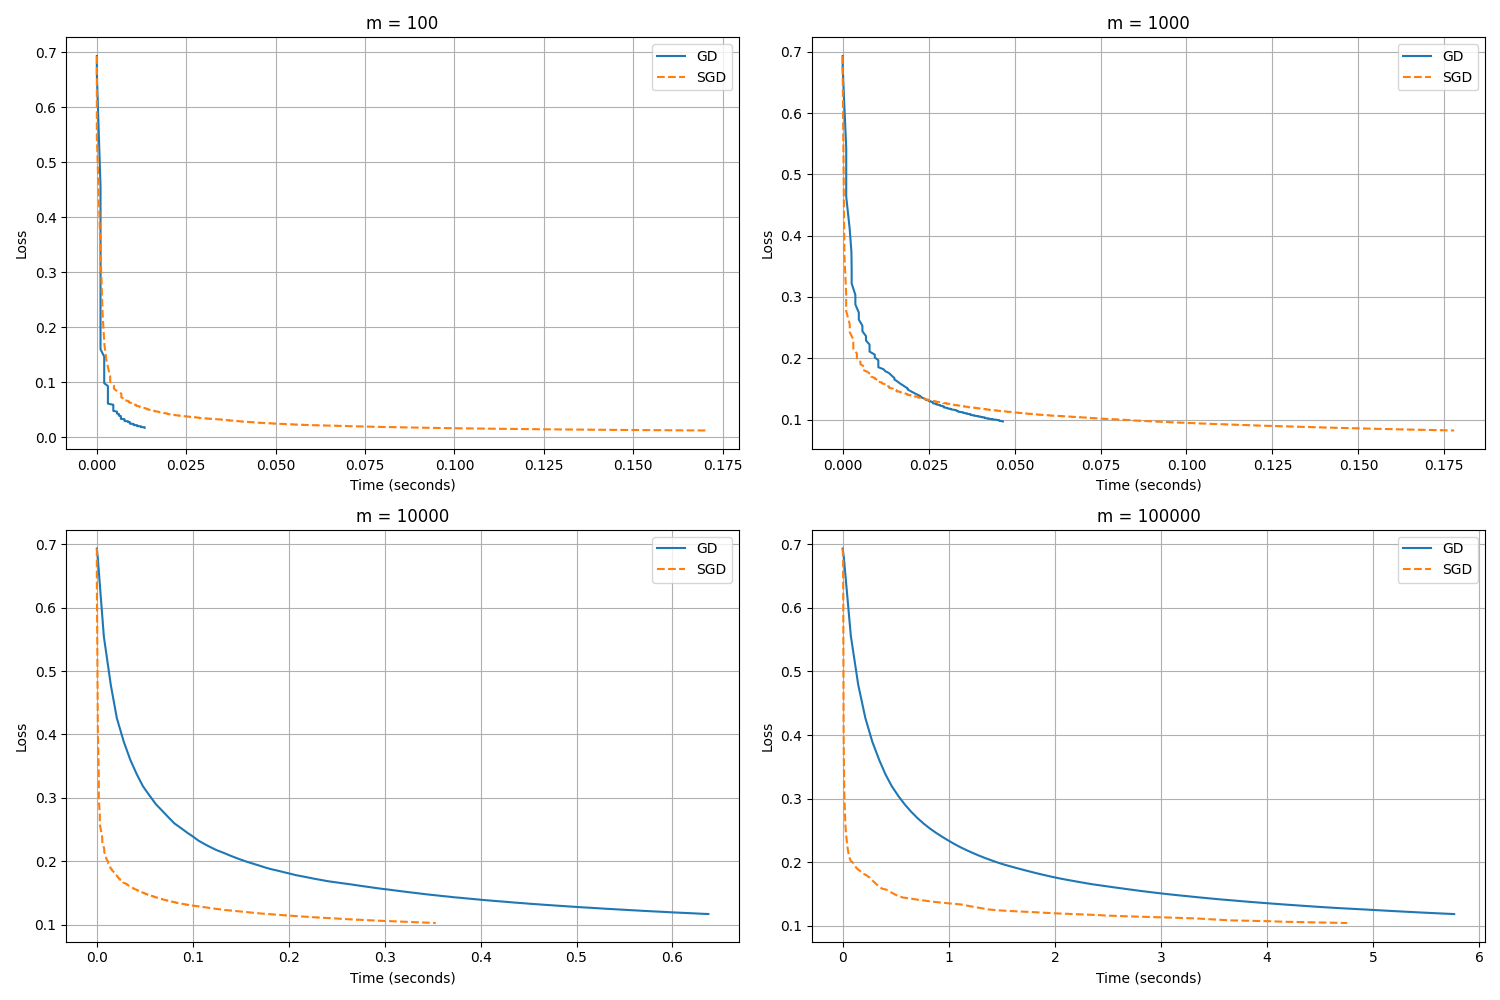
\includegraphics[width=0.8\textwidth]{p5_4.png}
	\caption{SGD vs. GD}
	\label{fig:p5_4}
	\end{figure}

\newpage
\section*{Problem 6 [15 pts]}
In class, we discussed Kernel SVM, we said there are many options for the kernel, such as linear, polynoimal, Gaussian, etc.
\begin{itemize}
	\item Show that if $K(i,j)=\frac{\langle \vx_i,\vx_j\rangle}{\|\vx_i\|_2\|\vx_j\|_2}$, then $K$ defines a proper kernel.
	\item We define $K=K_1+K_2$ where $K_1$ is Gaussian Kernel ($\gamma=1$) and $K_2$ is linear Kernel. Assume we are to train SVM on \href{https://en.wikipedia.org/wiki/Iris_flower_data_set}{iris} dataset using the kernel defined above ($K$). Since there are 3 classes, we need train 3 hyperplanes (one vs. one). Please determine how many support vectors for each of the 3 SVMs. (You can use quadratic programming solvers in Matlab or Python at your convinience)
\end{itemize}


\textcolor{red}{P6.1, Answer:}\\

To prove $K$ is a proper kernel, it must be symmetric and positive semi-definite.

First, for symmetry:
\[
K(i,j) = \frac{\langle \vx_i,\vx_j\rangle}{\|\vx_i\|_2\|\vx_j\|_2} = \frac{\langle \vx_j,\vx_i\rangle}{\|\vx_j\|_2\|\vx_i\|_2} = K(j,i)
\]

For positive semi-definiteness, let $\{\vx_1,\ldots,\vx_n\}$ be any set of vectors and $\{c_1,\ldots,c_n\}$ be any real coefficients. Define normalized vectors $\vy_i = \frac{\vx_i}{\|\vx_i\|_2}$. Then:

\[\sum_{i=1}^n\sum_{j=1}^n c_ic_jK(i,j) = \sum_{i=1}^n\sum_{j=1}^n c_ic_j\frac{\langle \vx_i,\vx_j\rangle}{\|\vx_i\|_2\|\vx_j\|_2} = \sum_{i=1}^n\sum_{j=1}^n c_ic_j\langle \vy_i,\vy_j\rangle = \left\|\sum_{i=1}^n c_i\vy_i\right\|_2^2 \geq 0\]

Therefore, $K$ is both symmetric and positive semi-definite, making it a proper kernel.\\

\textcolor{red}{P6.2, Answer:}\\

The optimization results for each binary classifier show using Python's CVXOPT quadratic programming solver:

\begin{figure}[h]
	\centering
	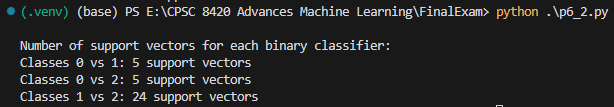
\includegraphics[width=0.8\textwidth]{p6_2.png}
	\caption{Support Vectors}
	\label{fig:p6_2}
	\end{figure}

Support vectors were counted as points where $\alpha_i > 10^{-5}$ in the optimal solution.
\begin{itemize}
    \item Setosa vs. Versicolor: 5 support vectors
    \item Setosa vs. Virginica: 5 support vectors
    \item Versicolor vs. Virginica: 24 support vectors
\end{itemize}



\newpage
\section*{Problem 7 [10 pts]}
\begin{itemize}
	\item Please tell me your favorite book, favorite travel destination and why.
	\item Please tell me the person who influences you most and why.
	\item Please tell me your favorite restaurant and dishes you order.
	\item Please tell me your favorite (or least favorite) part of this class.
	\item Please tell me your favorite machine learning algorithm(s) we discussed in class and why.
\end{itemize}


\textcolor{red}{P7.1, Answer:}\\

I have two favorite books. The first is The Count of Monte Cristo. It's just one of those timeless classics that really has everything. 
I like the French Revolution setting. I like the dramatic irony and how the author plays with character viewpoints. 
The second is For Whom the Bell Tolls. I guess I'm a sucker for adventure novels. I like that the book is about a time in history 
that we learn very little about in school. I like the characters and the story. It's part war hero story and part love story. It's just a great read.

As for traveling, I'm not a big traveler. I've been to the middle east for work (that isn't my favorite place). I've been to Mexico and the Carribean a few times,
and while they are great, it's more of just a fun tropical getaway. I would really like to go to Europe soon. 

If I had to pick a favorite place to travel, it would be the mountains. I enjoy going to western North Carolina a few times a year. 

\textcolor{red}{P7.2, Answer:}\\

I'd say my favorite person who has influenced me most is my wife. She's been a great partner and friend. She has helped me grow so much as a person.

\textcolor{red}{P7.3, Answer:}\\

My favorite restaurant is a little French restaurant in Charleston, SC called "Maison". They have really great entrees, but I really like their
wine pairing. They have great French pastries and Foie Gras. Definitely recommend it if you want a fancy dinner in Charleston.

\textcolor{red}{P7.4, Answer:}\\

My favorite part of the class is the depth in which you cover the machine learning models. I've taken a lot of machine learning courses, and this 
one has gone much deeper into the inner workings of the models. There were times when I felt I was way underprepared mathematically, but it was 
a great learning experience.

\textcolor{red}{P7.5, Answer:}\\

I'd say my favorite machine learning algorithm is probably PCA. I like the idea of reducing the dimensionality of the data and the idea of 
finding the principal components. I also like the idea of using the SVD to find the principal components. It's quite beautiful how it works.

\appendix
\section{Code Implementation}

\subsection{Problem 1.2: Convergence of Coordinate Descent}
\begin{verbatim}
import numpy as np
import matplotlib.pyplot as plt

def soft_threshold(x, lambda_):
    return np.sign(x) * np.maximum(np.abs(x) - lambda_, 0)

def coordinate_descent_lasso(X, y, lambda_, max_iter=1000, tol=1e-6):
    n, p = X.shape
    beta = np.random.randn(p)
    X_squared = np.sum(X ** 2, axis=0)
    objectives = []
    
    obj_init = 0.5 * np.sum((y - np.dot(X, beta)) ** 2) + lambda_ * np.sum(np.abs(beta))
    objectives.append(obj_init)
    
    for iter in range(max_iter):
        beta_old = beta.copy()
        
        for j in range(p):
            r = y - np.dot(X, beta)
            r = r + X[:, j] * beta[j]
            rho = np.dot(X[:, j], r)
            beta[j] = soft_threshold(rho, lambda_) / (X_squared[j] + 1e-10)
        
        obj = 0.5 * np.sum((y - np.dot(X, beta)) ** 2) + lambda_ * np.sum(np.abs(beta))
        objectives.append(obj)
        
        if np.max(np.abs(beta - beta_old)) < tol:
            print(f"Converged after {iter+1} iterations")
            break

    return beta, objectives

np.random.seed(42)
n, p = 100, 20
X = np.random.randn(n, p)
true_beta = np.random.randn(p)
y = np.dot(X, true_beta) + np.random.randn(n) * 0.1

Xty = np.dot(X.T, y)
Xty_inf_norm = np.max(np.abs(Xty))

lambda_ = 1.1 * Xty_inf_norm

print(f"||X^T * y||_inf = {Xty_inf_norm:.6f}")
print(f"lambda = {lambda_:.6f}")

beta_opt, objectives = coordinate_descent_lasso(X, y, lambda_)

print("\nOptimal beta:")
print(beta_opt)
print(f"\nMax absolute value in beta: {np.max(np.abs(beta_opt)):.6e}")

plt.figure(figsize=(10, 5))
plt.plot(range(len(objectives)), objectives, 'b-', linewidth=2)
plt.xlabel('Iteration')
plt.ylabel('Objective Value')
plt.title('Convergence of Coordinate Descent')
plt.yscale('log')
plt.grid(True)
plt.tight_layout()
plt.show()
\end{verbatim}


\subsection{Problem 3.1: PCA Biplot of US Arrests Data}
\begin{verbatim}
 import pandas as pd
import numpy as np
from sklearn.preprocessing import StandardScaler
import matplotlib.pyplot as plt

data = pd.read_csv("USArrests.csv")
states = data.iloc[:,0]
features = ["Murder", "Assault", "UrbanPop", "Rape"]

scaler = StandardScaler()
X = data[features]
X_scaled = scaler.fit_transform(X)

X_centered = X_scaled - np.mean(X_scaled, axis=0)
n_samples = X_scaled.shape[0]

cov_matrix = np.dot(X_centered.T, X_centered) / n_samples
eigenvals, eigenvecs = np.linalg.eig(cov_matrix)

pc1 = eigenvecs[:, 0]
pc2 = eigenvecs[:, 1]

proj_pc1 = np.dot(X_centered, pc1)
proj_pc2 = np.dot(X_centered, pc2)

plt.figure(figsize=(10, 8))
plt.xlim(-3.5, 3.5)
plt.ylim(-3.5, 3.5)

for i in range(len(states)):
    plt.text(proj_pc1[i], proj_pc2[i], states[i])

for i in range(len(features)):
    plt.arrow(0, 0, 
              pc1[i] * 3, pc2[i] * 3, 
              head_width=0.05, 
              head_length=0.05, 
              color='red')
    plt.annotate(features[i],
                xy=(pc1[i] * 3.5, pc2[i] * 3.5),
                xytext=(20, -20),
                textcoords='offset pixels', 
                color='red')

plt.grid(True)
plt.title('PCA Biplot of US Arrests Data')
plt.xlabel('First Principal Component')
plt.ylabel('Second Principal Component')
plt.show() 
\end{verbatim}

\subsection{Problem 3.2: Objective Function vs Iteration for 4 Features}
\begin{verbatim}
import pandas as pd
import numpy as np
from sklearn.preprocessing import StandardScaler
import matplotlib.pyplot as plt

data = pd.read_csv("USArrests.csv")
states = data.iloc[:,0]
features = ["Murder", "Assault", "UrbanPop", "Rape"]

scaler = StandardScaler()
X = data[features]
X_scaled = scaler.fit_transform(X)

mask = np.ones_like(X_scaled)
for i in range(len(states)):
    mask[i, np.random.randint(0, 4)] = 0

def nuclear_prox(Z, tau):
    U, s, Vt = np.linalg.svd(Z, full_matrices=False)
    s = np.maximum(s - tau, 0)
    return U @ np.diag(s) @ Vt

def objective(X, Z, mask, lambda_=1.0):
    return 0.5 * np.sum((mask * (X - Z))**2) + np.sum(np.linalg.svd(Z, compute_uv=False))

Z = np.zeros_like(X_scaled)
step_size = 1.0
max_iter = 100
obj_values = []

for iter in range(max_iter):
    grad = mask * (Z - X_scaled)
    Z_new = Z - step_size * grad
    Z_new = nuclear_prox(Z_new, step_size)
    
    obj = objective(X_scaled, Z_new, mask)
    obj_values.append(obj)
    
    if iter > 0 and abs(obj_values[-1] - obj_values[-2]) < 1e-6:
        break
    
    Z = Z_new

plt.figure(figsize=(10, 5))
plt.plot(obj_values, 'b-')
plt.xlabel('Iteration')
plt.ylabel('Objective Value')
plt.title('Objective Function vs Iteration')
plt.grid(True)
plt.show()
\end{verbatim}

\subsection{Problem 4: Spectral Clustering}
\begin{verbatim}
import numpy as np
import matplotlib.pyplot as plt
from matplotlib.colors import ListedColormap
from sklearn.cluster import KMeans
from sklearn.neighbors import kneighbors_graph

def generate_concentric_data(n_points=150, noise=0.25):
    radii = [1.0, 2.8, 5.0]
    data = []
    labels = []
    
    for i, r in enumerate(radii):
        angles = np.random.uniform(0, 2*np.pi, n_points)
        x = r * np.cos(angles) + np.random.normal(0, noise, n_points)
        y = r * np.sin(angles) + np.random.normal(0, noise, n_points)
        data.extend(list(zip(x, y)))
        labels.extend([i] * n_points)
    
    return np.array(data), np.array(labels)

def compute_knn_similarity(X, k=10):
    A = kneighbors_graph(X, n_neighbors=k, mode='connectivity', include_self=False)
    A = A.toarray()
    W = np.maximum(A, A.T)
    return W

def spectral_clustering(X, k_neighbors=10, n_clusters=3):
    W = compute_knn_similarity(X, k=k_neighbors)
    
    D = np.diag(np.sum(W, axis=1))
    D_inv_sqrt = np.diag(1.0 / np.sqrt(np.sum(W, axis=1)))
    L = np.eye(W.shape[0]) - D_inv_sqrt @ W @ D_inv_sqrt
    
    eigenvals, eigenvecs = np.linalg.eigh(L)
    idx = np.argsort(eigenvals)
    eigenvals = eigenvals[idx]
    eigenvecs = eigenvecs[:, idx]
    
    Y = eigenvecs[:, 1:3]
    Y = Y / np.sqrt(np.sum(Y**2, axis=1))[:, np.newaxis]
    
    kmeans = KMeans(n_clusters=n_clusters, n_init=50, random_state=42)
    labels = kmeans.fit_predict(Y)
    
    centers = np.zeros((n_clusters, 2))
    for i in range(n_clusters):
        mask = labels == i
        centers[i] = np.mean(X[mask], axis=0)
    radii = np.sqrt(np.sum(centers**2, axis=1))
    order = np.argsort(radii)
    new_labels = np.zeros_like(labels)
    for i, old_label in enumerate(order):
        new_labels[labels == old_label] = i
    
    return new_labels, eigenvals, eigenvecs

np.random.seed(42)
X, true_labels = generate_concentric_data()
labels, eigenvals, eigenvecs = spectral_clustering(X)

colors = ['orange', 'skyblue', 'lightgreen']
custom_cmap = ListedColormap(colors)

fig, axs = plt.subplots(2, 2, figsize=(12, 12))

axs[0,0].scatter(X[:,0], X[:,1], c=labels, cmap=custom_cmap)
axs[0,0].set_title('Data and Clustering')
axs[0,0].set_xlim(-6, 6)
axs[0,0].set_ylim(-6, 6)

axs[0,1].plot(range(1, 16), eigenvals[1:16], 'go-')
axs[0,1].set_title('Eigenvalues')

n_points = len(X)
axs[1,0].set_title('Eigenvectors')
axs[1,0].set_xlabel('Index')
axs[1,0].set_ylabel('2nd/3rd Smallest')

axs[1,0].scatter(range(n_points), eigenvecs[:, 1], c=labels, cmap=custom_cmap, s=10, alpha=0.6)
axs[1,0].scatter(range(n_points), eigenvecs[:, 2], c=labels, cmap=custom_cmap, s=10, alpha=0.6)
axs[1,0].axhline(y=0, color='black', linestyle='--', alpha=0.5)
axs[1,0].set_ylim(-0.1, 0.1)
axs[1,0].set_xlim(0, 450)

axs[1,1].scatter(eigenvecs[:, 1], eigenvecs[:, 2], c=labels, cmap=custom_cmap)
axs[1,1].set_title('Spectral Clustering')

plt.tight_layout()
plt.show() 	
\end{verbatim}







\subsection{Problem 5.1: Gradient Descent for Logistic Regression}
\begin{verbatim}
import numpy as np
import matplotlib.pyplot as plt

np.random.seed(42)
m = 100
n = 100

X = np.random.randn(m, n) 
w_true = np.random.randn(n)
prob = 1 / (1 + np.exp(-X @ w_true))
y_01 = (prob > 0.5).astype(float)
y_pm = 2 * y_01 - 1

def gradient_descent_pm(X, y, w_init, lr=0.01, max_iter=1000):
    w = w_init.copy()
    losses = []
    
    for i in range(max_iter):
        z = y * (X @ w)
        pred = 1 / (1 + np.exp(z))
        loss = np.mean(np.log(1 + np.exp(-z)))
        grad = -X.T @ (y * pred) / m
            
        w = w - lr * grad
        losses.append(loss)
    
    return w, losses

def gradient_descent_01(X, y, w_init, lr=0.01, max_iter=1000):
    w = w_init.copy()
    losses = []
    
    for i in range(max_iter):
        z = X @ w
        pred = 1 / (1 + np.exp(-z))
        loss = -np.mean(y * np.log(pred + 1e-10) + (1-y) * np.log(1 - pred + 1e-10))
        grad = X.T @ (pred - y) / m
            
        w = w - lr * grad
        losses.append(loss)
    
    return w, losses

w_init = np.zeros(n)

w_pm, losses_pm = gradient_descent_pm(X, y_pm, w_init)
w_01, losses_01 = gradient_descent_01(X, y_01, w_init)

plt.figure(figsize=(10, 5))
plt.plot(losses_pm, label='{-1,+1} formulation')
plt.plot(losses_01, '--', label='{0,1} formulation')
plt.xlabel('Iteration')
plt.ylabel('Loss')
plt.title('Loss vs Iteration for Both Formulations')
plt.legend()
plt.grid(True)

weight_diff = np.linalg.norm(w_pm - w_01)
print(f"L2 norm of weight difference: {weight_diff:.6f}")
print(f"Weights for ±1: {w_pm}")
print(f"Weights for 0/1: {w_01}")

plt.show()
\end{verbatim}

\subsection{Problem 5.2: MSE vs Cross-Entropy for Logistic Regression}
\begin{verbatim}
import numpy as np
import matplotlib.pyplot as plt

np.random.seed(42)
n_samples = 100
X = np.random.randn(n_samples, 2)
w_true = np.array([2.0, -1.0])
p_true = 1 / (1 + np.exp(-X @ w_true))
y = (p_true > 0.5).astype(float)

def sigmoid(x):
    return 1 / (1 + np.exp(-x))

def gradient_descent_mse(X, y, w_init, lr=0.1, max_iter=1000):
    w = w_init.copy()
    losses = []
    probs = []
    
    for i in range(max_iter):
        p = sigmoid(X @ w)
        loss = 0.5 * np.mean((y - p)**2)
        grad = -X.T @ ((y - p) * p * (1-p)) / len(y)
        
        w = w - lr * grad
        losses.append(loss)
        probs.append(p[0])
    
    return w, losses, probs

def gradient_descent_ce(X, y, w_init, lr=0.1, max_iter=1000):
    w = w_init.copy()
    losses = []
    probs = []
    
    for i in range(max_iter):
        p = sigmoid(X @ w)
        loss = -np.mean(y * np.log(p + 1e-10) + (1-y) * np.log(1 - p + 1e-10))
        grad = X.T @ (p - y) / len(y)
        
        w = w - lr * grad
        losses.append(loss)
        probs.append(p[0])
    
    return w, losses, probs

w_init = np.array([-10.0, -10.0])

w_mse, losses_mse, probs_mse = gradient_descent_mse(X, y, w_init)
w_ce, losses_ce, probs_ce = gradient_descent_ce(X, y, w_init)

plt.figure(figsize=(12, 5))

plt.subplot(121)
plt.plot(losses_mse, label='MSE')
plt.plot(losses_ce, label='Cross-Entropy')
plt.xlabel('Iteration')
plt.ylabel('Loss')
plt.title('Loss vs Iteration')
plt.legend()
plt.grid(True)

plt.subplot(122)
plt.plot(probs_mse, label='MSE')
plt.plot(probs_ce, label='Cross-Entropy')
plt.xlabel('Iteration')
plt.ylabel('Probability (p)')
plt.title('Probability Evolution for First Sample')
plt.legend()
plt.grid(True)

plt.tight_layout()
plt.show()

print(f"Final probability (MSE): {probs_mse[-1]:.6f}")
print(f"Final probability (CE): {probs_ce[-1]:.6f}")
\end{verbatim}


\subsection{Problem 5.3: Newton's Method for Logistic Regression}
\begin{verbatim}
import numpy as np
import matplotlib.pyplot as plt

np.random.seed(42)
m = 100
n = 100

X = np.random.randn(m, n)
w_true = np.random.randn(n)
prob = 1 / (1 + np.exp(-X @ w_true))
y = (prob > 0.5).astype(float)

def sigmoid(x):
    # Clip values for numerical stability
    x = np.clip(x, -700, 700)
    return 1 / (1 + np.exp(-x))

def gradient_descent(X, y, w_init, lr=0.1, max_iter=1000):
    w = w_init.copy()
    losses = []
    
    for i in range(max_iter):
        z = X @ w
        p = sigmoid(z)
        loss = -np.mean(y * np.log(p + 1e-10) + (1-y) * np.log(1 - p + 1e-10))
        grad = X.T @ (p - y) / m
        
        w = w - lr * grad
        losses.append(loss)
    
    return w, losses

def newton_method(X, y, w_init, max_iter=1000):
    w = w_init.copy()
    losses = []
    
    # Small regularization to prevent singular Hessian
    lambda_reg = 1e-5
    I = np.eye(n)
    
    for i in range(max_iter):
        z = X @ w
        p = sigmoid(z)
        loss = -np.mean(y * np.log(p + 1e-10) + (1-y) * np.log(1 - p + 1e-10))
        grad = X.T @ (p - y) / m
        
        # Compute Hessian with regularization
        S = np.diag((p * (1-p)).flatten())
        H = X.T @ S @ X / m + lambda_reg * I
        
        # Newton update with unit stepsize
        w = w - np.linalg.solve(H, grad)
        losses.append(loss)
    
    return w, losses

w_init = np.zeros(n)

w_gd, losses_gd = gradient_descent(X, y, w_init)
w_newton, losses_newton = newton_method(X, y, w_init)

plt.figure(figsize=(10, 5))
plt.plot(losses_gd, label='Gradient Descent')
plt.plot(losses_newton, label='Newton Method')
plt.xlabel('Iteration')
plt.ylabel('Loss')
plt.title('Loss vs Iteration')
plt.legend()
plt.grid(True)
plt.show() 

\end{verbatim}

\subsection{Problem 5.4: SGD vs GD for Logistic Regression}
\begin{verbatim}
import numpy as np
import matplotlib.pyplot as plt
import time

def sigmoid(x):
    x = np.clip(x, -700, 700)
    return 1 / (1 + np.exp(-x))

def generate_data(m, n):
    X = np.random.randn(m, n)
    w_true = np.random.randn(n)
    prob = 1 / (1 + np.exp(-X @ w_true))
    y = (prob > 0.5).astype(float)
    return X, y

def batch_gradient_descent(X, y, w_init, lr=0.1, max_iter=1000):
    start_time = time.time()
    w = w_init.copy()
    times = [0]
    losses = [compute_loss(X, y, w)]
    
    for i in range(max_iter):
        p = sigmoid(X @ w)
        grad = X.T @ (p - y) / len(y)
        w = w - lr * grad
        
        if i % 10 == 0:
            times.append(time.time() - start_time)
            losses.append(compute_loss(X, y, w))
    
    return w, times, losses

def stochastic_gradient_descent(X, y, w_init, max_iter=5000):
    start_time = time.time()
    w = w_init.copy()
    times = [0]
    losses = [compute_loss(X, y, w)]
    batch_size = 32
    
    for t in range(max_iter):
        indices = np.random.choice(len(y), batch_size)
        x_batch = X[indices]
        y_batch = y[indices]
        
        lr = 1.0 / np.sqrt(t + 1)
        p = sigmoid(x_batch @ w)
        grad = x_batch.T @ (p - y_batch) / batch_size
        w = w - lr * grad
        
        if t % 10 == 0:
            times.append(time.time() - start_time)
            losses.append(compute_loss(X, y, w))
    
    return w, times, losses

def compute_loss(X, y, w):
    p = sigmoid(X @ w)
    return -np.mean(y * np.log(p + 1e-10) + (1-y) * np.log(1 - p + 1e-10))

n = 100
sample_sizes = [100, 1000, 10000, 100000]

plt.figure(figsize=(15, 10))
for i, m in enumerate(sample_sizes, 1):
    np.random.seed(42)
    X, y = generate_data(m, n)
    w_init = np.zeros(n)
    
    _, times_gd, losses_gd = batch_gradient_descent(X, y, w_init)
    _, times_sgd, losses_sgd = stochastic_gradient_descent(X, y, w_init)
    
    plt.subplot(2, 2, i)
    plt.plot(times_gd, losses_gd, label='GD')
    plt.plot(times_sgd, losses_sgd, '--', label='SGD')
    plt.xlabel('Time (seconds)')
    plt.ylabel('Loss')
    plt.title(f'm = {m}')
    plt.legend()
    plt.grid(True)

plt.tight_layout()
plt.show()

\end{verbatim}

\subsection{Problem 6.2: Support Vector Machines}


\begin{verbatim}
import numpy as np
from sklearn.datasets import load_iris
from cvxopt import matrix, solvers
from sklearn.preprocessing import StandardScaler
solvers.options['show_progress'] = False

iris = load_iris()
X = StandardScaler().fit_transform(iris.data)
y = iris.target

def compute_kernel(x1, x2, gamma=1.0):
    gaussian = np.exp(-gamma * np.sum((x1 - x2)**2))
    linear = np.dot(x1, x2)
    return gaussian + linear

def train_svm(X, y, C=1.0):
    n_samples = len(X)
    
    K = np.zeros((n_samples, n_samples))
    for i in range(n_samples):
        for j in range(n_samples):
            K[i,j] = compute_kernel(X[i], X[j])
    
    y = y.astype(float)
    
    P = matrix(np.outer(y, y) * K)
    q = matrix(-np.ones(n_samples))
    G = matrix(np.vstack((-np.eye(n_samples), np.eye(n_samples))))
    h = matrix(np.hstack((np.zeros(n_samples), C*np.ones(n_samples))))
    A = matrix(y.reshape(1, -1).astype(float))
    b = matrix(np.zeros(1))
    
    solution = solvers.qp(P, q, G, h, A, b)
    alphas = np.array(solution['x']).flatten()
    
    sv = alphas > 1e-5
    return np.sum(sv)

print("\nNumber of support vectors for each binary classifier:")
for i in range(3):
    for j in range(i+1, 3):
        mask = np.logical_or(y == i, y == j)
        X_sub = X[mask]
        y_sub = y[mask]
        y_sub = np.where(y_sub == i, 1, -1)
        
        n_sv = train_svm(X_sub, y_sub)
        print(f"Classes {i} vs {j}: {n_sv} support vectors")
\end{verbatim}




\end{document}
